\documentclass[12pt, A4]{report}
\usepackage[utf8]{inputenc}
\usepackage{ragged2e}
\usepackage{graphicx}
\usepackage[a4paper, total={6in, 8in}]{geometry}
\usepackage{media9}
\usepackage[utf8]{inputenc}
\usepackage[T1]{fontenc}
\usepackage{parskip}
\usepackage{tabulary}
\usepackage{hyperref}
\usepackage{fontawesome}

\begin{document}
\begin{center}
    \huge{Computer Science Lab Report}\\[10pt]
    \large{Hassan Muhammad Yousuf}
\end{center}


\tableofcontents
\newpage

\section{Abstract}

\rule{\textwidth}{0.1pt}
    \noindent 
    \justifying This report contains several solutions based on exercises. The solved exercises demonstrate how students can use various tools to work more efficiently and effectively. In addition to this, The report emphasizes the application of various techniques in the solved word-problems being taught in the computer science lab module, that includes the reduction of typing effort, while highlighting the utilization of essential tools such as LaTeX for formal document preparation, Linux for open source server management system, HTML and CSS for web development, Jupyter for interactive coding, and Git and GitHub for small and large projects to control and collaboration. Through the incorporation of a variety of tools, the study not only identifies solutions to computer science problems, but also provides insights on how to maximize the efficacy of tools in computer science-related work. This form of integration identifies the most efficient and effective methods for resolving a specific problem. It also gives a framework for figuring out how to get the most out of these tools, which may improve the accuracy and speed learning of the students with which one completes work in the field of computer science.
\newpage
\section{Introduction}

\rule{\textwidth}{0.1pt}
    \noindent 
    \justifying Field related to  \textbf{Information technology} increasing and evolving rapidly, because the  \textbf{Global Market} demands well trained professionals in this area which plays  crucial role in shaping  \textbf{Modern  World}. The purpose of writing this report is to overview the comprehensive and various exercises taught in  \textbf{Computer  Science  Lab} which include multiple skills we will discuss blow. the report will highlight the key features of each exercises done in lab along with their  \textbf{Coding  Models} and  \textbf{Visual Shots}.

\subsection{Touch Typing}
\rule{\textwidth}{0.1pt}
\subsubsection{Introduction}
Touch Typing is a style of typing which is used to perform multiple task using via input device with less brain involvement because the location of keys are stored in the Muscle Memory. Touch Typing is also called blind typing.

\subsubsection{Explanation}
The Purpose of this exercise is to develop the skills in the students of effortless typing. The figure shows the progress of typing skills of the author of this report.
\begin{figure}[htb!]
\centering
\textbf{\caption{Touch Typing Progress}}
  \includegraphics[scale = 1.5]{Progress.png}
\end{figure}\\
\newpage
\subsection{Latex}
\rule{\textwidth}{0.1pt}
\subsubsection{Introduction}
Latex is a system of document preparation which was markup tagging convection to define the general structure of a documents. latex is widely used in document preparation such as project reports, thesis and much more in multiple fields for instance Computer Science, Physics, Engineering, Linguistics e.t.c. it also plays crucial role in preparation of books and articles that contain multilingual materials. Latex uses the TEX Typesetting program for formatting its output and is itself written in the TEX Macro language.

\subsubsection{Explanation}
The purpose of this exercise is to enable the author work on markup documentation. Latex gives the user extremely good control over the formatting of documents. In this exercise author of this report develop his Resume using Latex System. the visualization of the Output as well as background coding is attached as blow.
\subsubsection{Output}

\begin{figure}[htb!]
\centering
\textbf{\caption{Latex Resume}}
  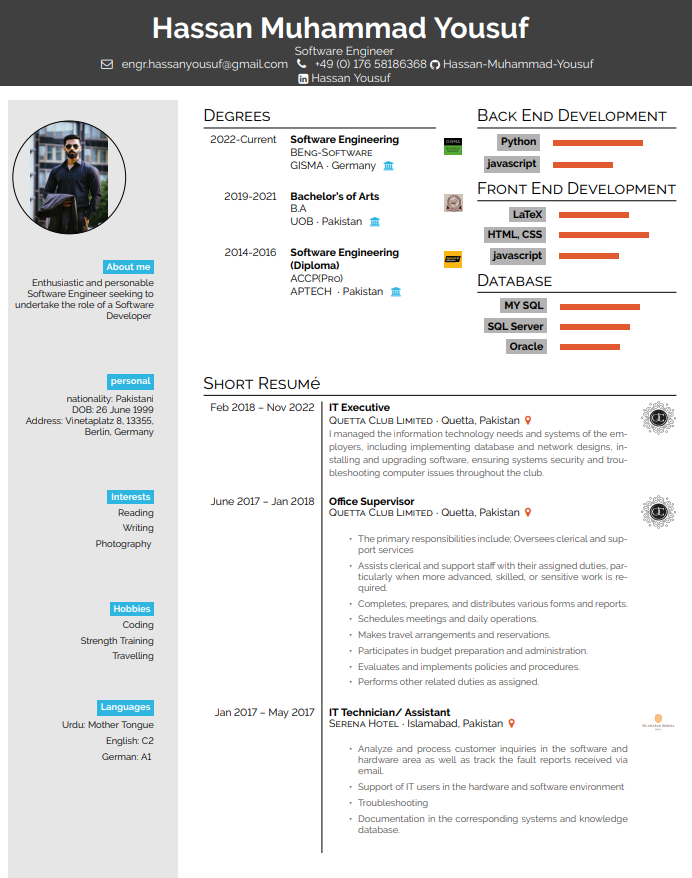
\includegraphics[width = 140 mm]{CV SS.png}
\end{figure}\\

\subsubsection{Background Coding}
\begin{figure}[htb!]
\centering
\textbf{\caption{Background Coding}}
  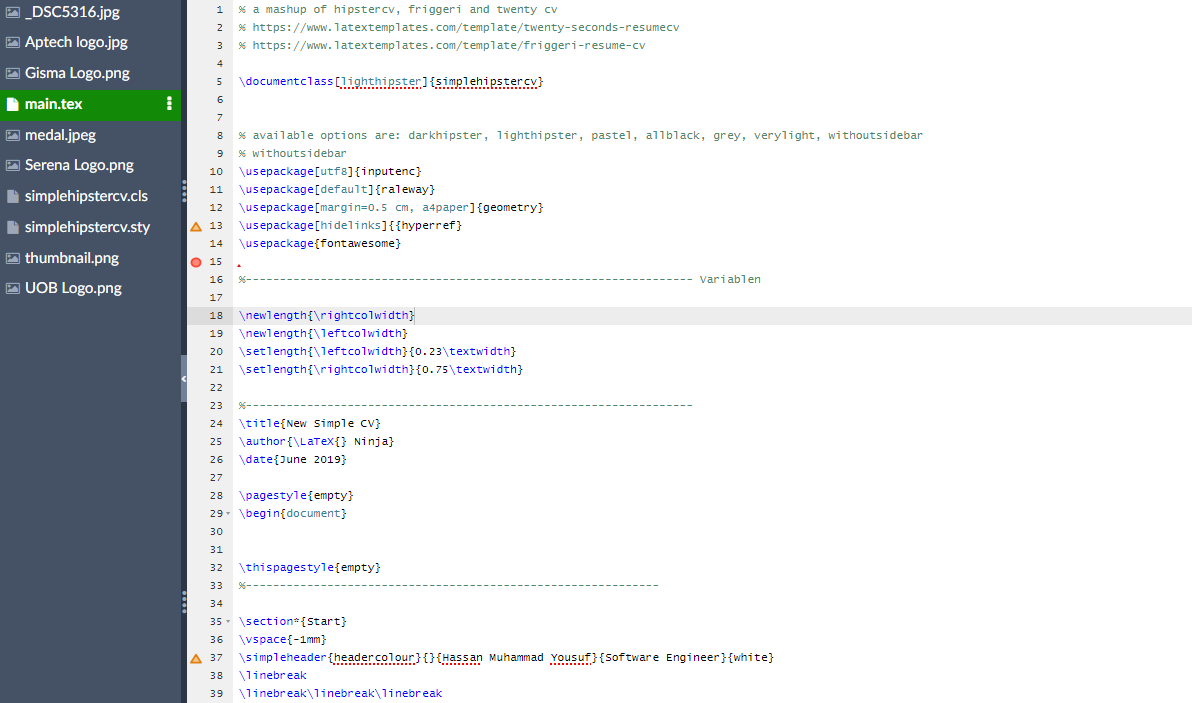
\includegraphics[width = 150 mm]{Bg Code.png}
\end{figure}\\
\begin{figure}[htb!]
\centering
\textbf{\caption{Background Coding}}
  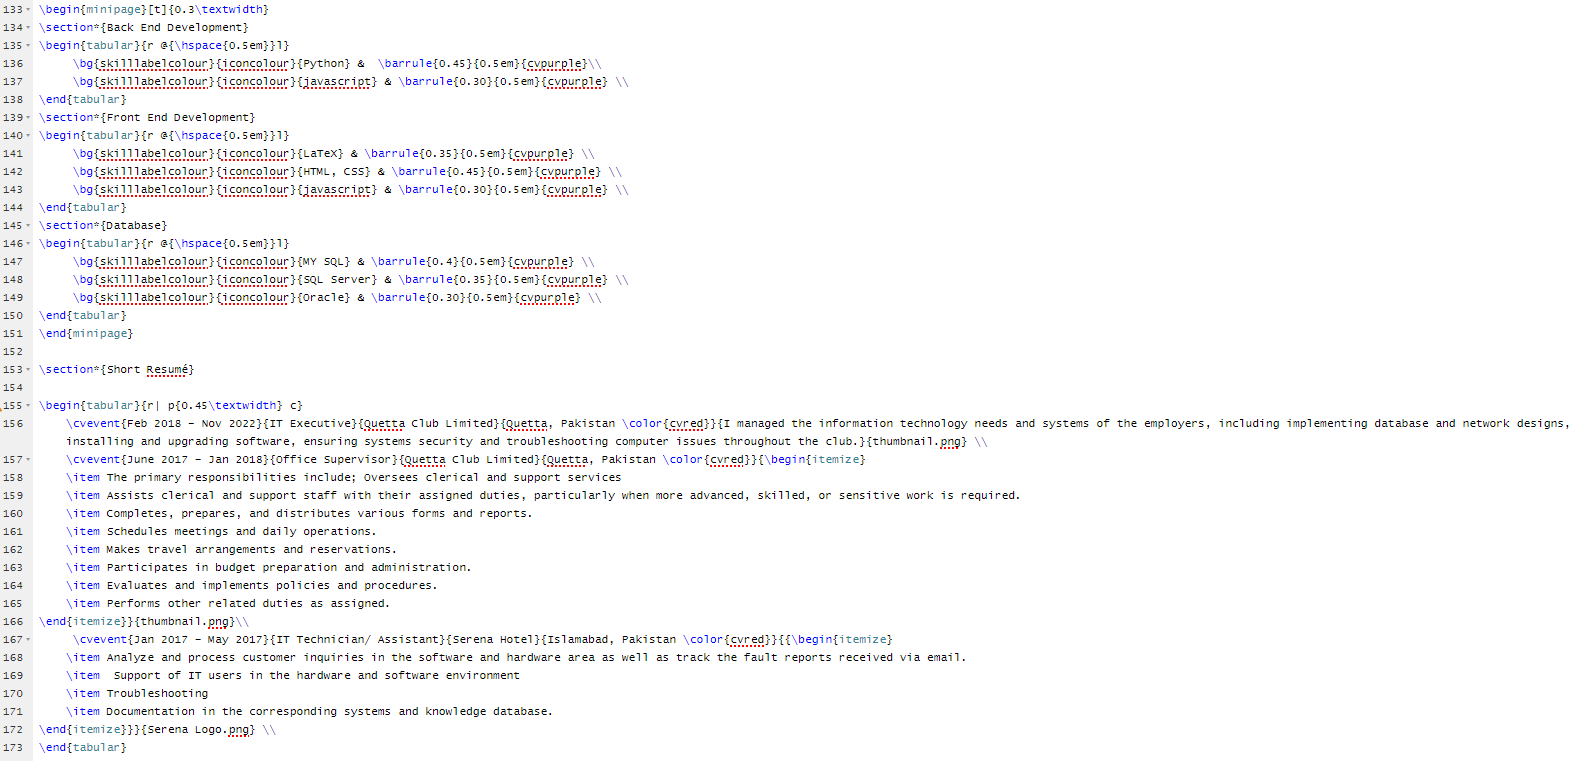
\includegraphics[width = 150 mm]{Bg Code 2.png}
\end{figure}\\
\subsection{Linux Shell}
\rule{\textwidth}{0.1pt}
\subsubsection{Introduction}
Linux is Open Source Operating System that is use similarly like Windows and \\Mac-OS. It is used for its multiple Key Features such as:
\begin{itemize}
    \item Open Source Platform
    \item Distribution
    \item Command Line Interface (CLI)
    \item Graphical User Interface (GUI)
    \item Multi User / Multitasking
    \item Security 
    \item Server Management
\end{itemize} 
Linux provide customized environment that empower user their specific needs.
\subsubsection{Explanation}
The purpose of this section is to enable author of this report works on Open Sources Operating System. In this exercise the author has used Virtual Box for operating Linux on Windows along with Putty(terminal emulator) which enable user to transfer files from multiple Operating System running on same machine. In this exercise author has also demonstrate the usage of Command Line Interface and creates digital clock by using Script Shell. Results are displayed blow.
\subsubsection{Output}
\includemedia[width=1\linewidth,height=0.4\linewidth,activate=pageopen,
passcontext,
transparent,
addresource=Report Recording 3.mp4,
flashvars={source=Report Recording 3.mp4}
]{
\includegraphics[width=0.6\linewidth]{Adobe SS.png}}{VPlayer.swf}
\subsubsection{Background Coding}
\begin{tabular}{cc}
  \includegraphics[height=0.30\textheight]{Report SS Linux 1.png}
  &
  \includegraphics[height=0.30\textheight]{Report SS.png}
   \\                                                     
   
 \end{tabular}

\subsection{HTML & CSS}
\rule{\textwidth}{0.1pt}
\subsubsection{Introduction}
HTML (Hyper Text Markup Language) and CSS (Cascading Style Sheets) are the basic blocks of building web pages. HTML provides the structure of page and CSS look out visual layouts. HTML and CSS are the foundations of web development and considered as back bone in modern world. Usage of these technologies are adapted and supported widely. Mastering HTML and CSS enables you to gain solid foundation for building web technologies.
\subsubsection{Explanation}
In this exercise the author has created his web portfolio using HTML and CSS. The author has also used JavaScript in the contact form to maintain the record of person who drop the message. Author has also create responsive layout by using CSS. The purpose of this profile is to show the detailed overview of the author projects and personal blog-spot. Here are some visual shots of Web Profile and background coding attached under:
\subsubsection{Output}
\includemedia[width=1\linewidth,height=0.4\linewidth,activate=pageopen,
passcontext,
transparent,
addresource=output.mp4,
flashvars={source=output.mp4}
]{
\includegraphics[width=0.6\linewidth]{Adobe SS.png}}{VPlayer.swf}
\subsubsection{Background Coding}
\begin{tabular}{cc}
  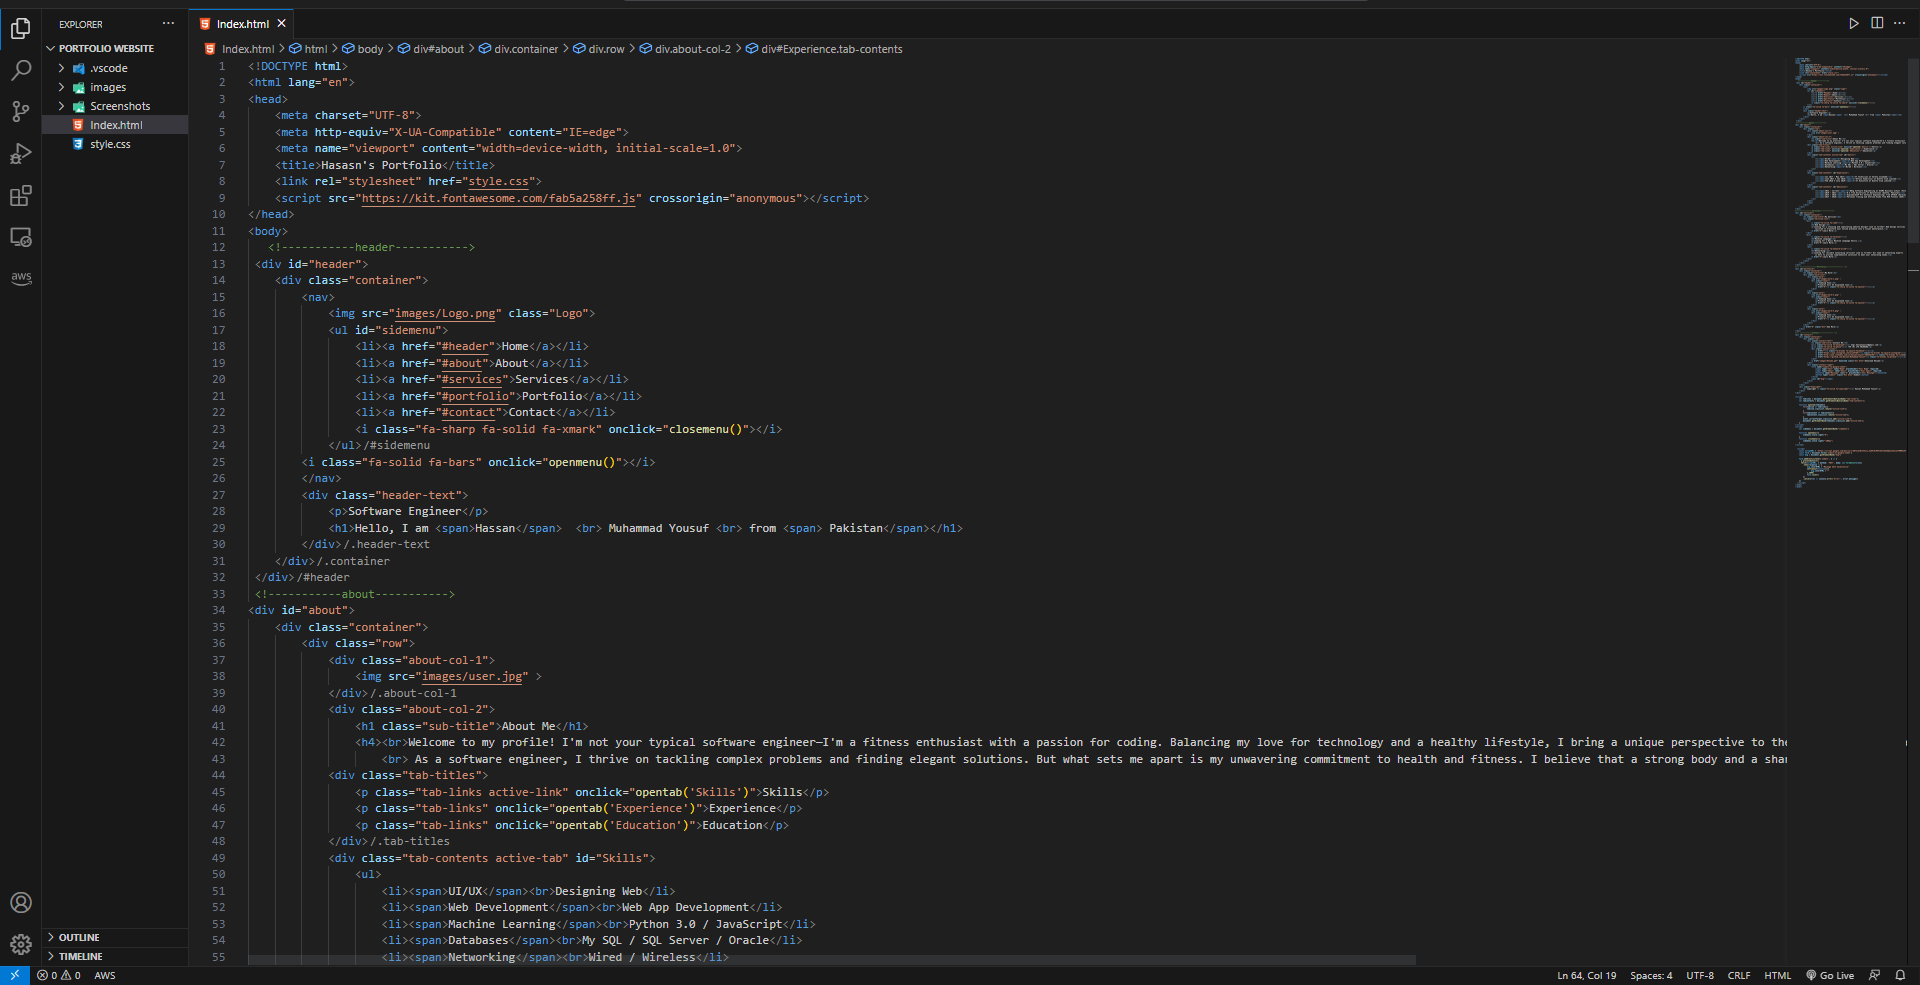
\includegraphics[width=225,height=0.20\textheight]{HTML Code.png}
  &
  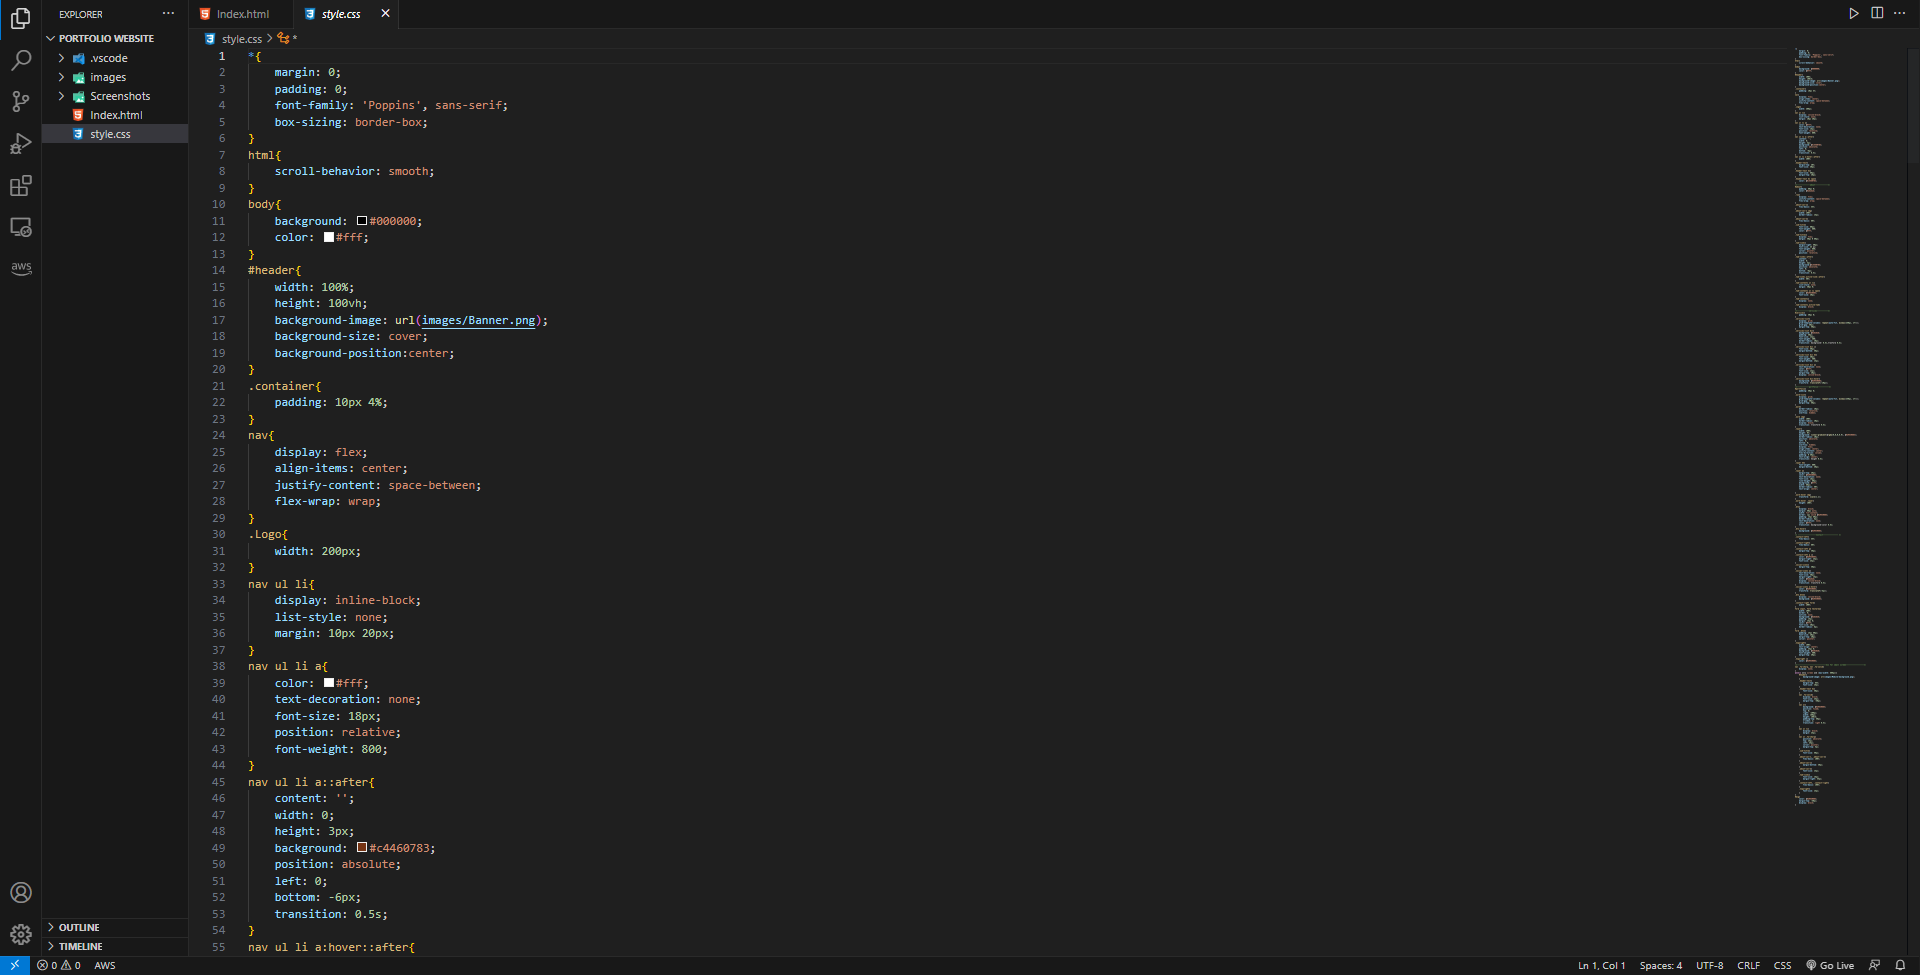
\includegraphics[width=225,height=0.20\textheight]{CSS Code.png}
 \\
  HTML Code & CSS Code
\end{tabular}

\begin{tabular}{cc}
  \includegraphics[width=225,height=0.20\textheight]{Responsive Layout.png}
  &
  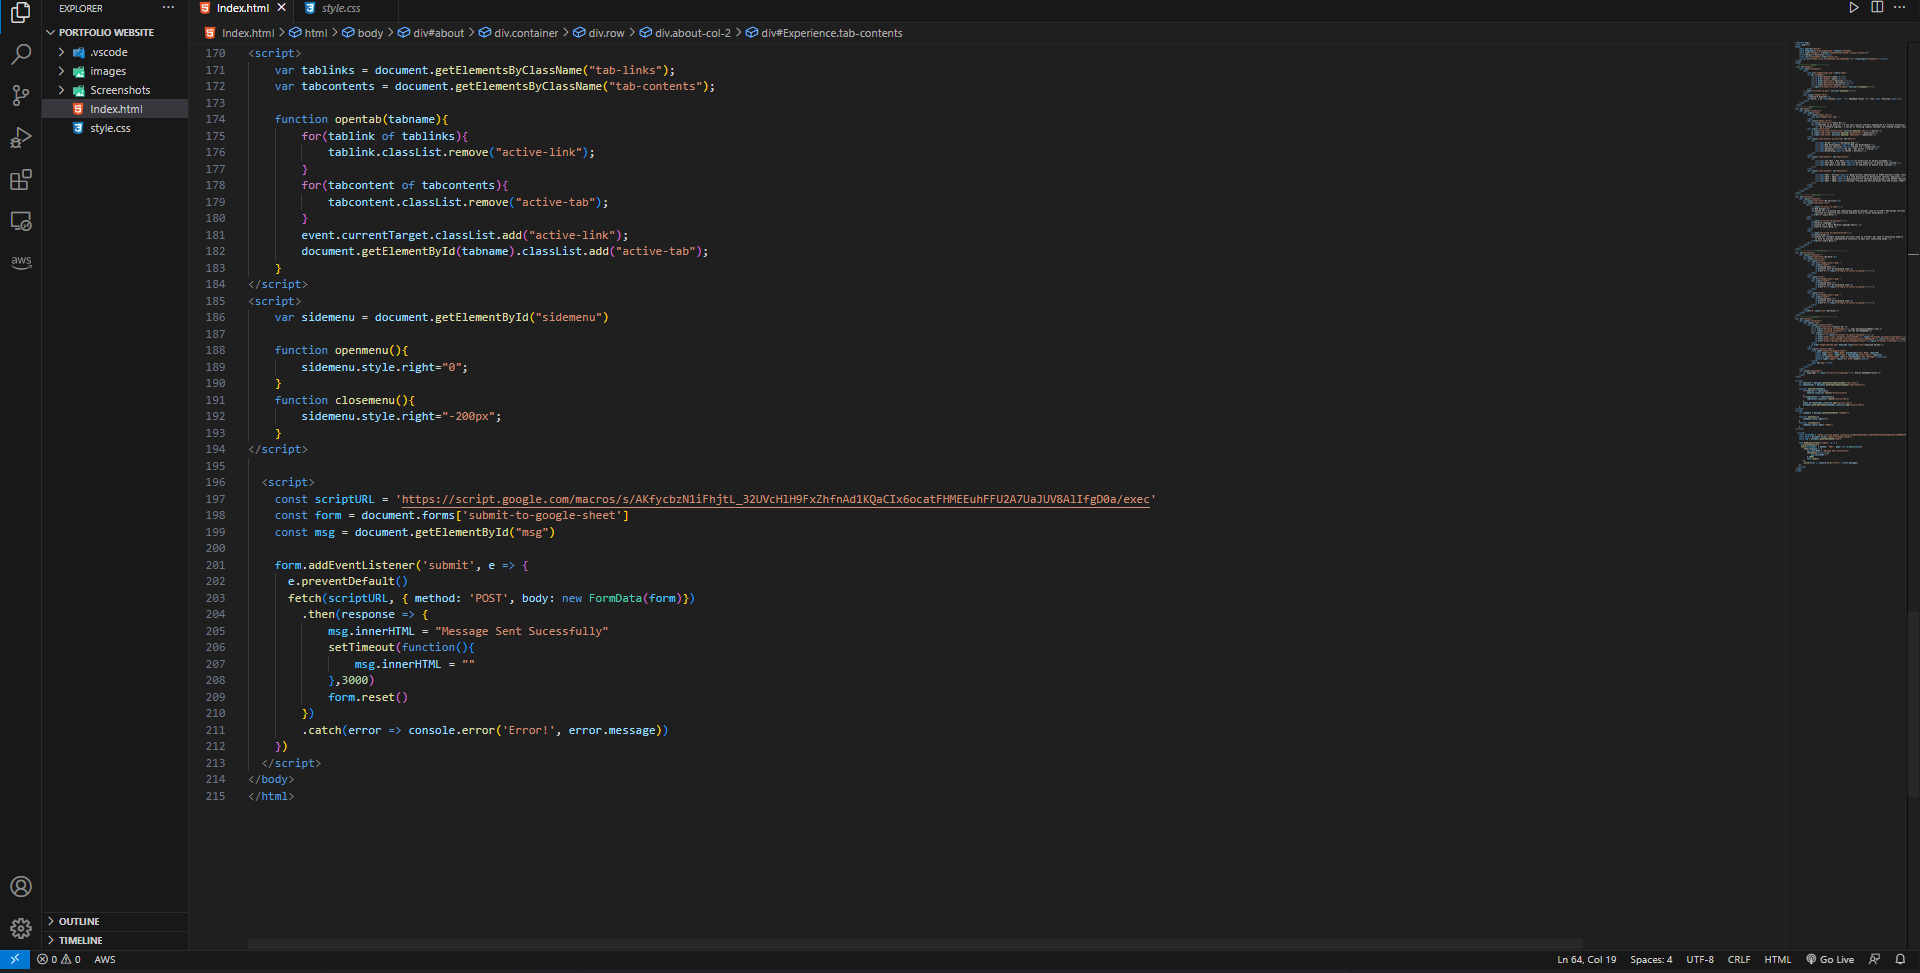
\includegraphics[width=225,height=0.20\textheight]{JS code.png}
   \\  
  JavaScript Code & CSS Responsive Layout Code
   
 \end{tabular}

\vspace{5mm}
\subsection{Juypter}
\rule{\textwidth}{0.1pt}
\subsubsection{Introduction}
The Jupyter Notebook is an open-source web application that allows users to create and share documents containing live code, equations, visualizations, and narrative prose. For example, it provides an environment for data scientists to develop and explore models and can also be used as a teaching platform for classes and workshops. Data cleansing and transformation, numerical simulation, statistical modeling, data visualization, and machine learning are only a few of the many applications. However, the Jupyter Notebook is not without its flaws. One of the most common complaints is that the Jupyter Notebook is slow and resource-intensive, which can make working with large datasets difficult. Additionally, because the Jupyter Notebook is a web-based application, it can be susceptible to security vulnerabilities. It also requires some technical expertise to set up and maintain, which can be a barrier for non-technical users. Finally, its open-source nature can lead to inconsistent user experiences, making it difficult for users to collaborate. Jupyter Notebook is capable of operating locally on your device as a local server or remotely on a server. Your browser is used to initiate a Jupyter notebook. Because it is possible to include live code and other complex text components such as equations, links, images, and tables, it is referred to as a notebook. Consequently, you can have a beautiful notebook that describes your concept and contains the live code in a single file. As a consequence, Jupyter notebooks have become a popular method for putting concepts to the test as well as for composing journals, papers, and even books; this book, for example, was written entirely within Jupyter notebooks. This article will only cover the fundamentals of the Jupyter notebook because we are just getting you started with it. Obviously, it has many more advantages. For instance, the Jupyter notebook allows you to easily share your work with others as it supports a variety of file formats, such as HTML, PDF, Markdown, and even LaTeX
\subsubsection{Explanation}
In this exercise the author will able to use Juypter notebook. In this exercise the reporter use Gapminder data collection to show data analytic of world population. Reporter shows different analysis of GDP and population using Plotly and Pandas graphical Representation. Reporter has also used Markdown cells to script the reports in the notebook. More details of this exercise is shown blow.
\subsubsection{Output}
\begin{tabular}{cc}
  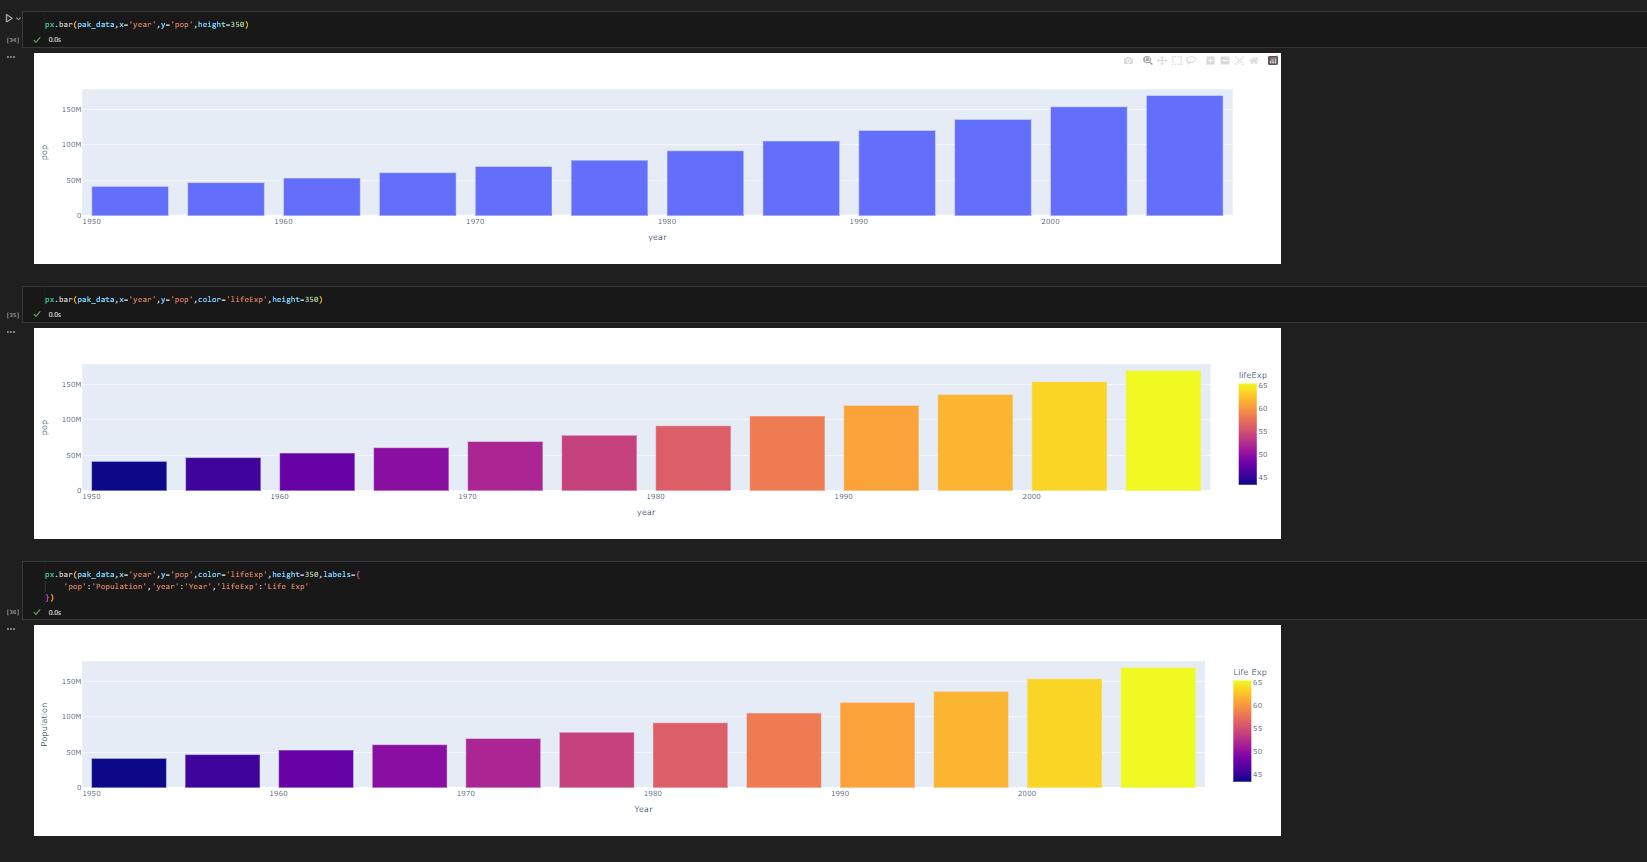
\includegraphics[width=225,height=0.20\textheight]{OP1.png}
  &
  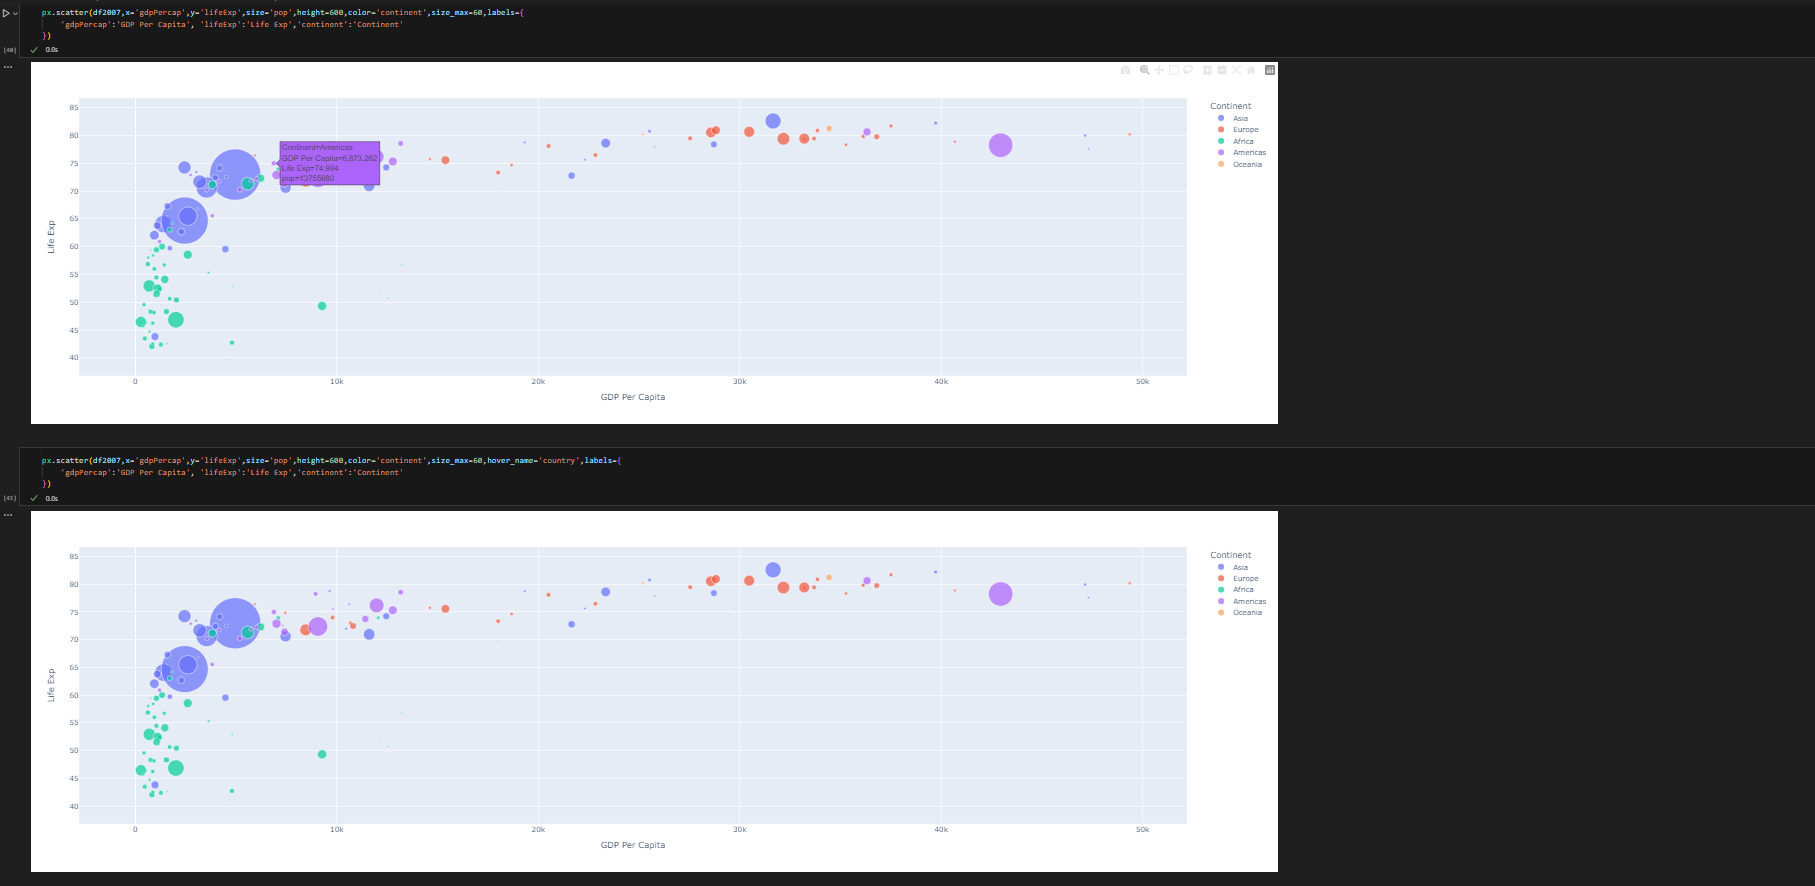
\includegraphics[width=225,height=0.20\textheight]{OP2.png}
  &
  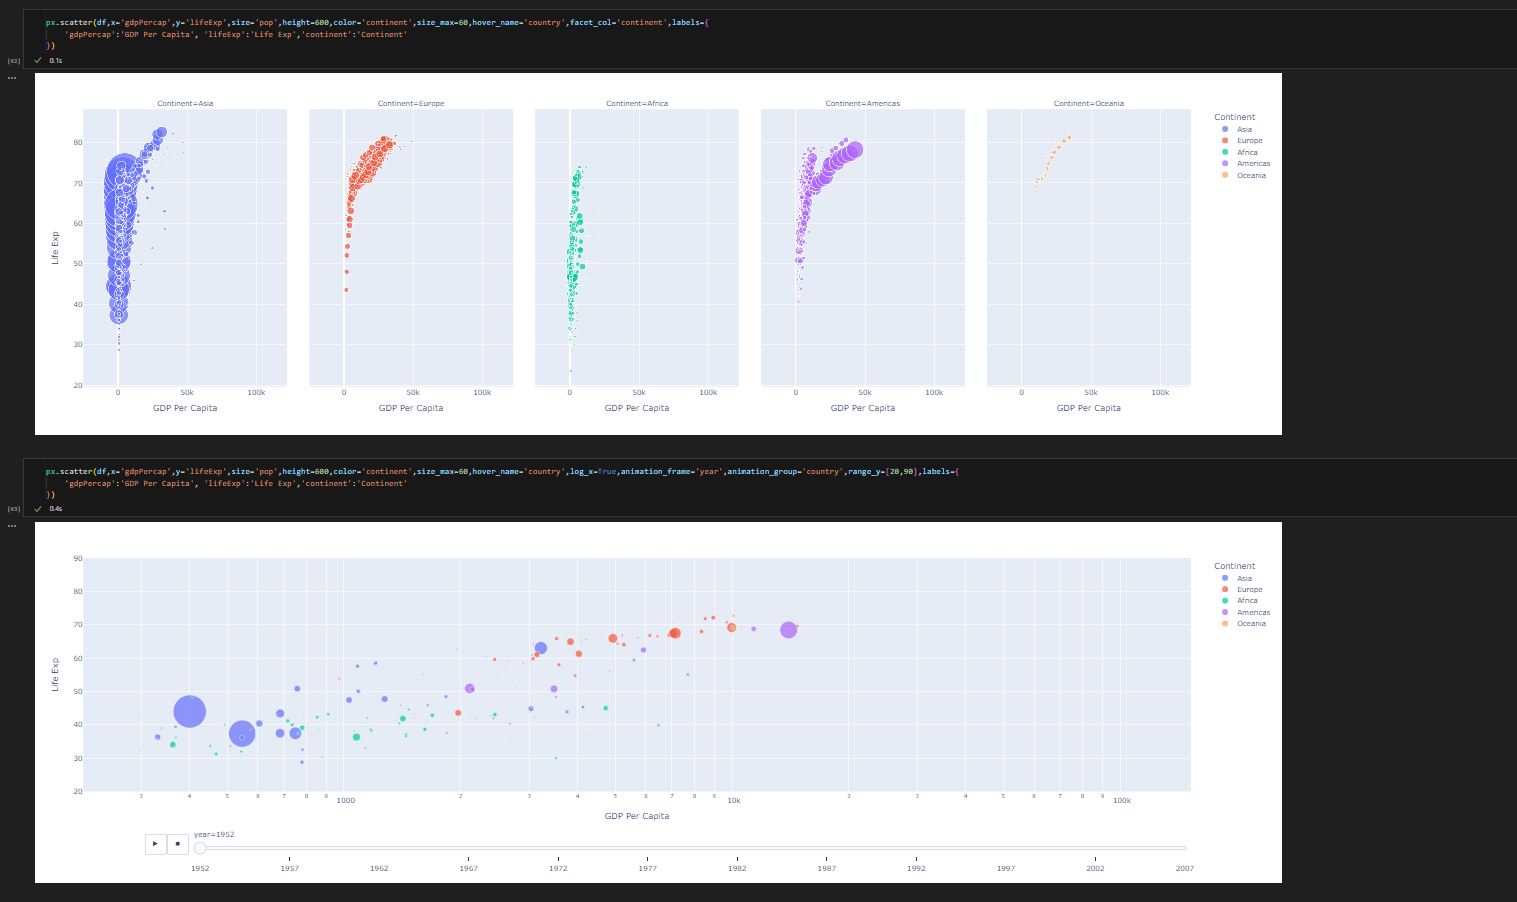
\includegraphics[width=225,height=0.20\textheight]{Op3.png}
  &
  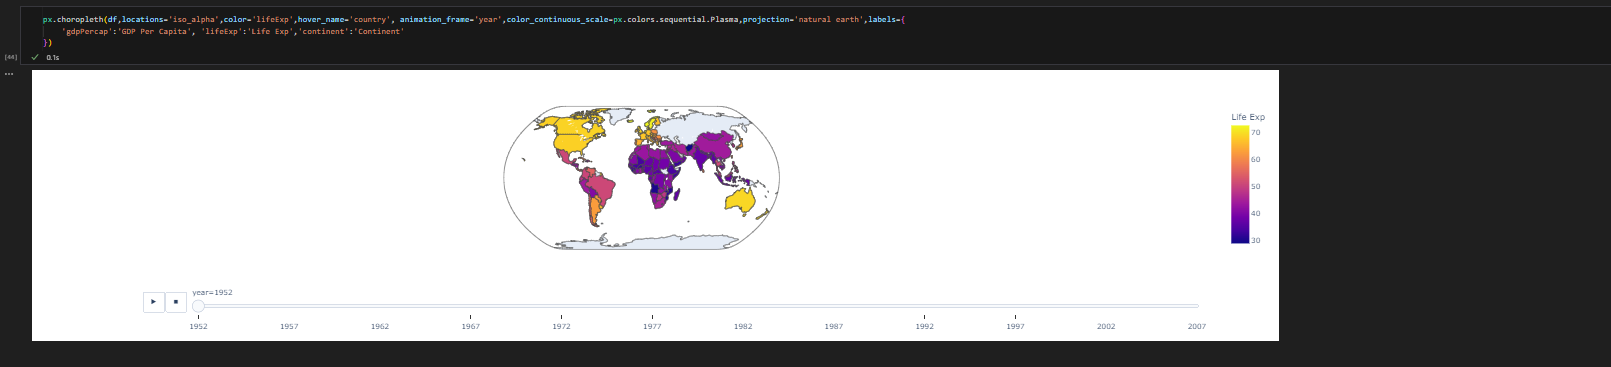
\includegraphics[width=225,height=0.20\textheight]{OP4.png}
 \end{tabular}

\subsubsection{Background Coding}
\begin{tabular}{cc}
  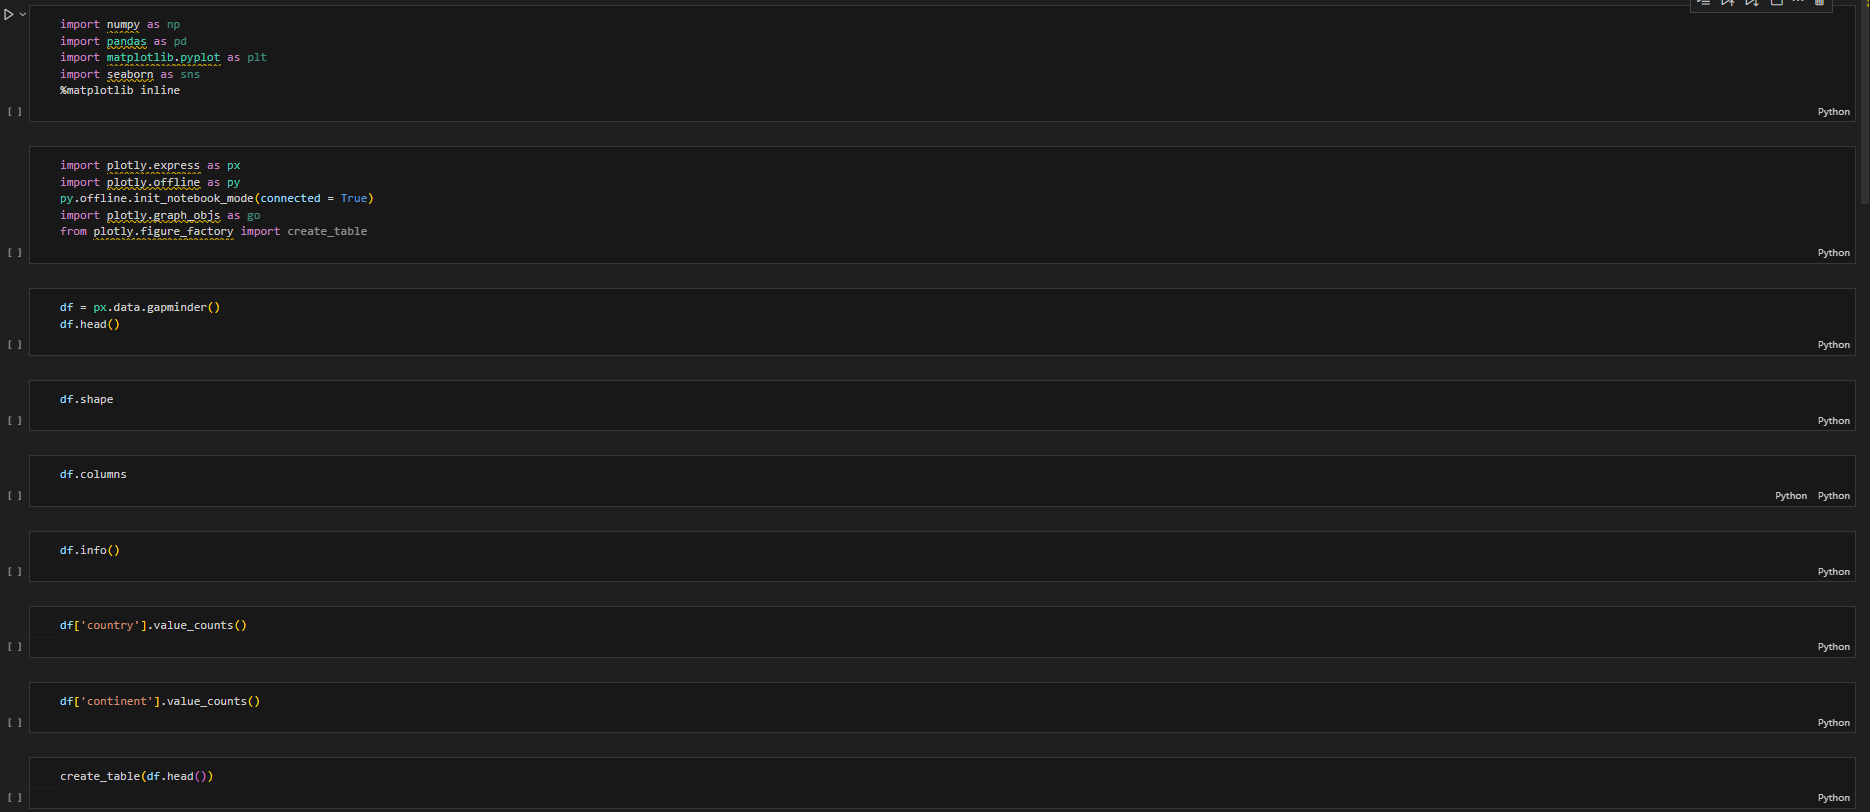
\includegraphics[width=225,height=0.20\textheight]{BG1.png}
  &
  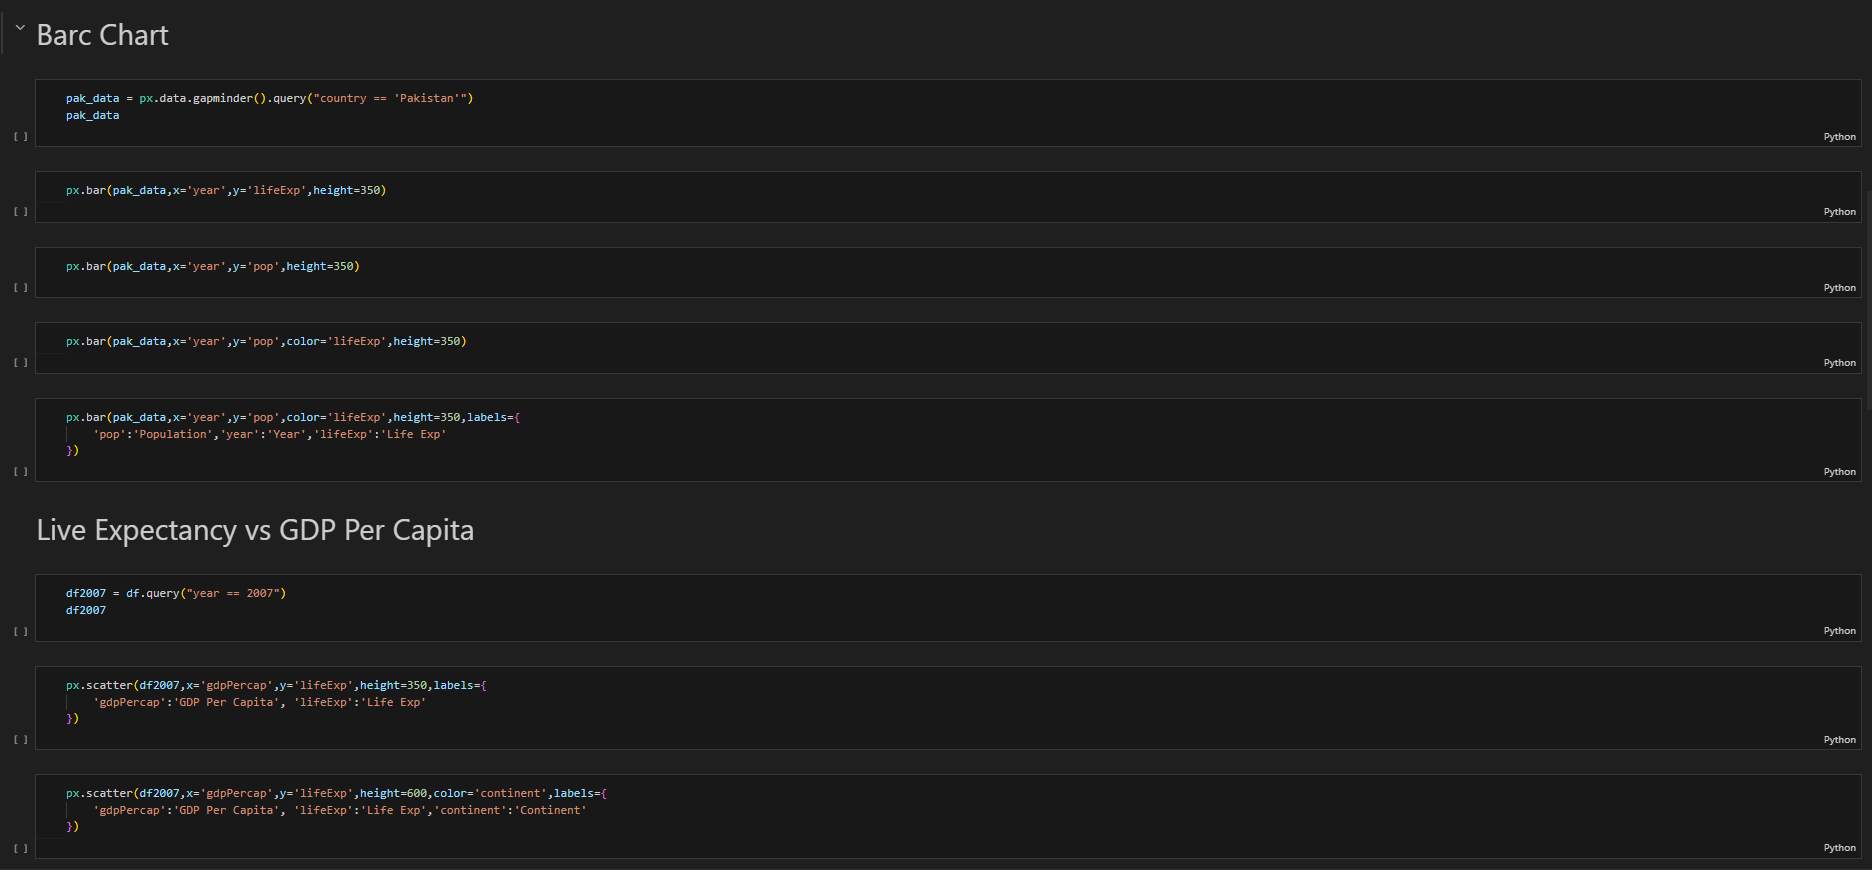
\includegraphics[width=225,height=0.20\textheight]{BG2.png}
  &
  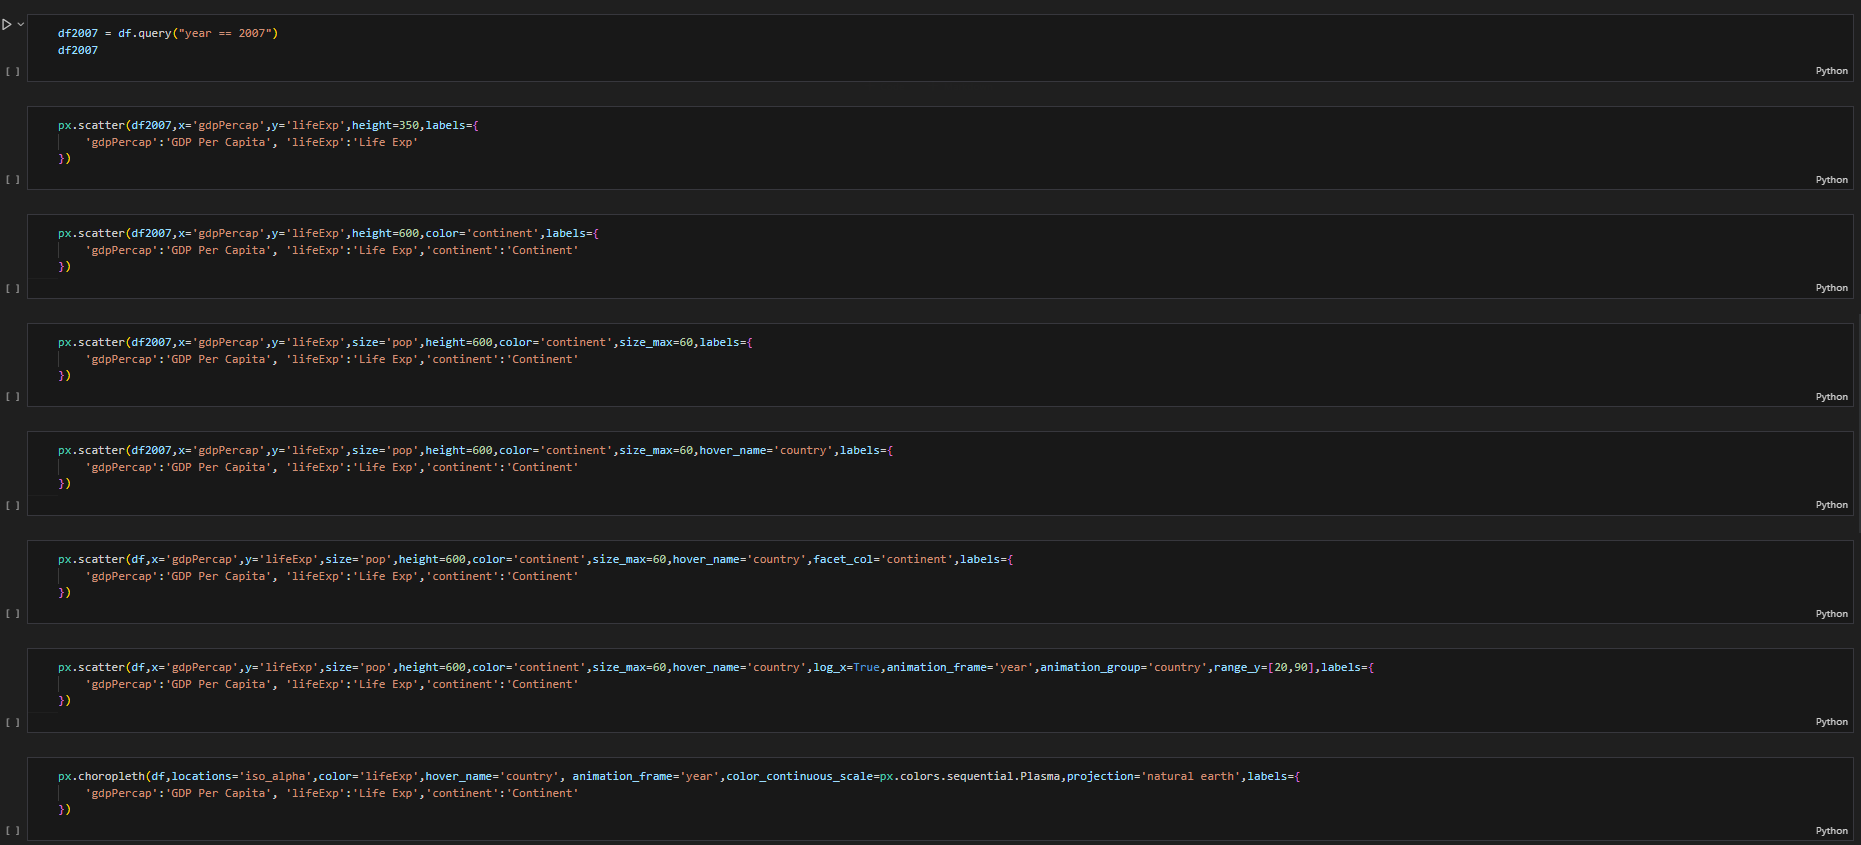
\includegraphics[width=225,height=0.20\textheight]{BG 3.png}
  &
  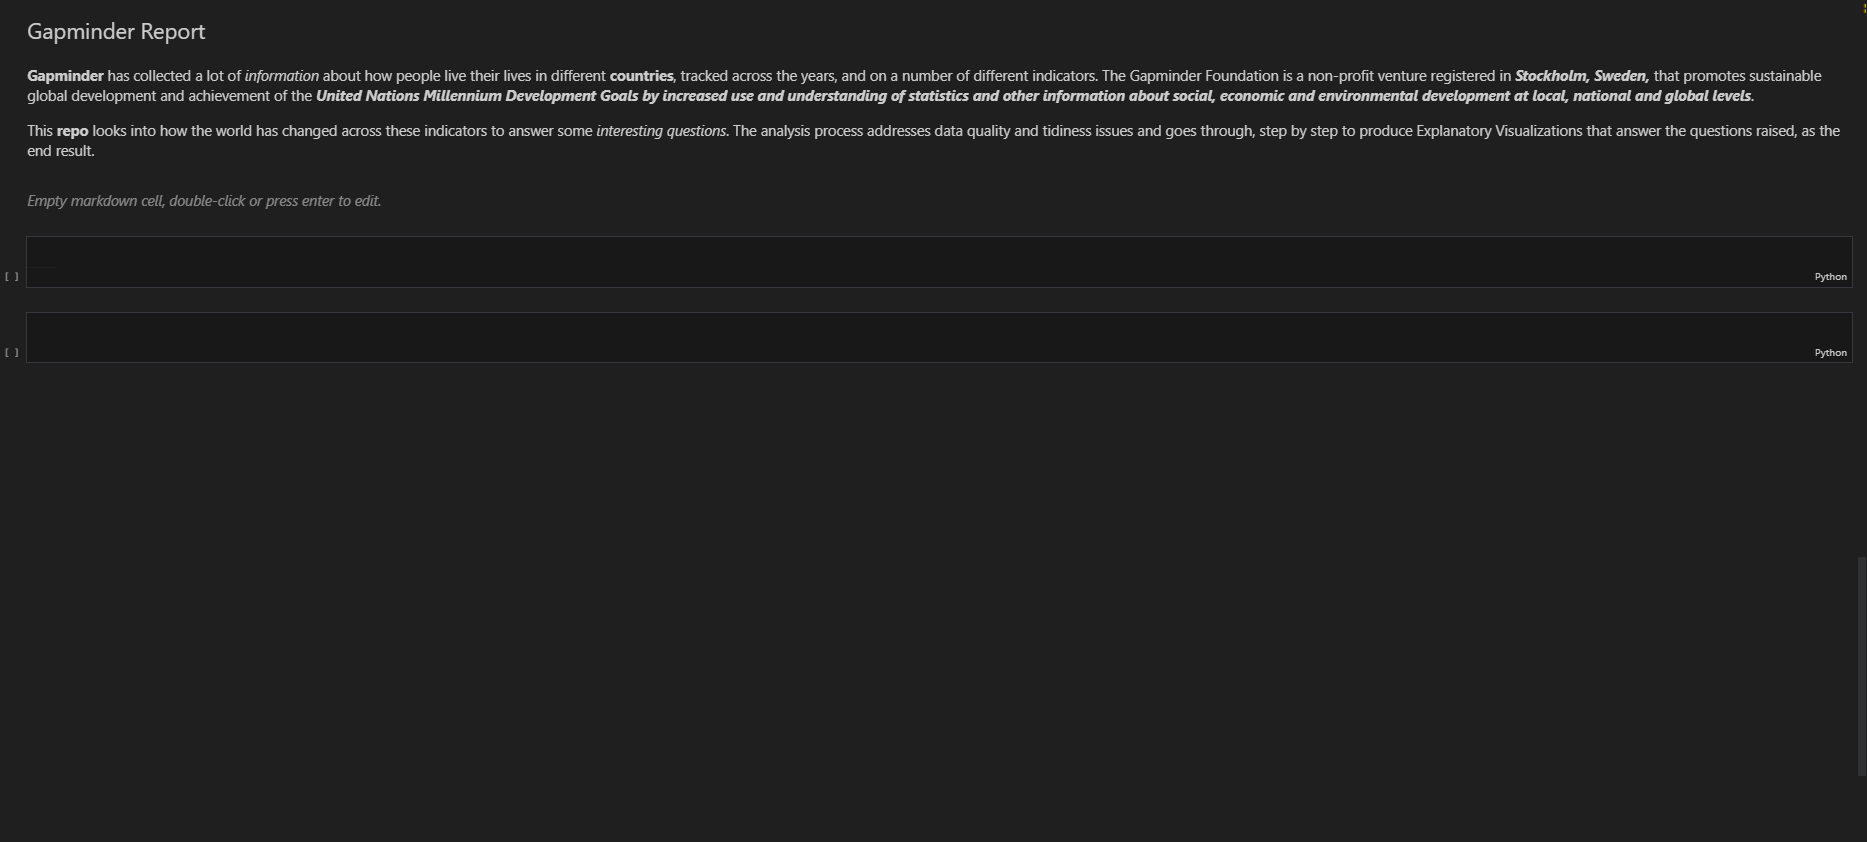
\includegraphics[width=225,height=0.20\textheight]{BG4.png}
 \end{tabular}
 
\subsection{Git}
\rule{\textwidth}{0.1pt}
\subsubsection{Introduction}
Git is a free and open source distributed version control system designed to handle everything from small to very large projects with speed and efficiency. Git is a mature, actively maintained open source project originally developed in 2005 by Linus Torvalds, the famous creator of the Linux operating system kernel. A staggering number of software projects rely on Git for version control, including commercial projects as well as open source. Developers who have worked with Git are well represented in the pool of available software development talent and it works well on a wide range of operating systems and IDEs (Integrated Development Environments).
\subsubsection{Explanation}
In this exercise the reporter has used git bash to create the repository in his machine which enable the reporter to manage the multiple platforms in one repository. The reporter has pushed all the exercise done in the module of Computer Science Lab trough the repository here is some visual screenshots of the coding structures blow.
\vspace{10mm}
\\
\begin{tabular}{cc}
  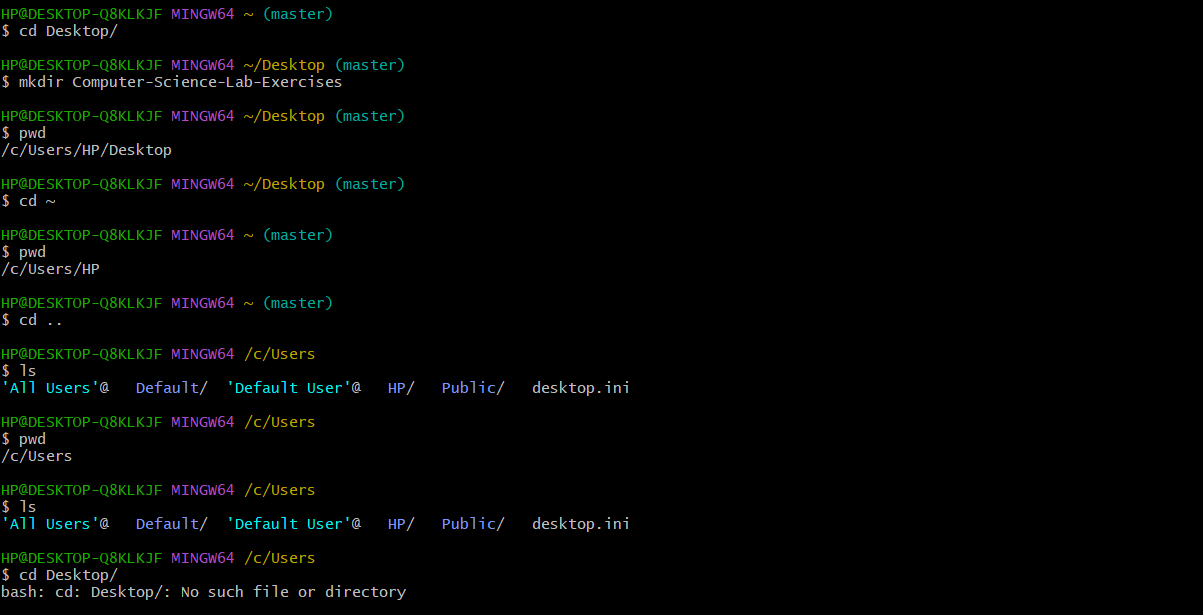
\includegraphics[width=225,height=0.35\textheight]{Git 1.png}
  &
  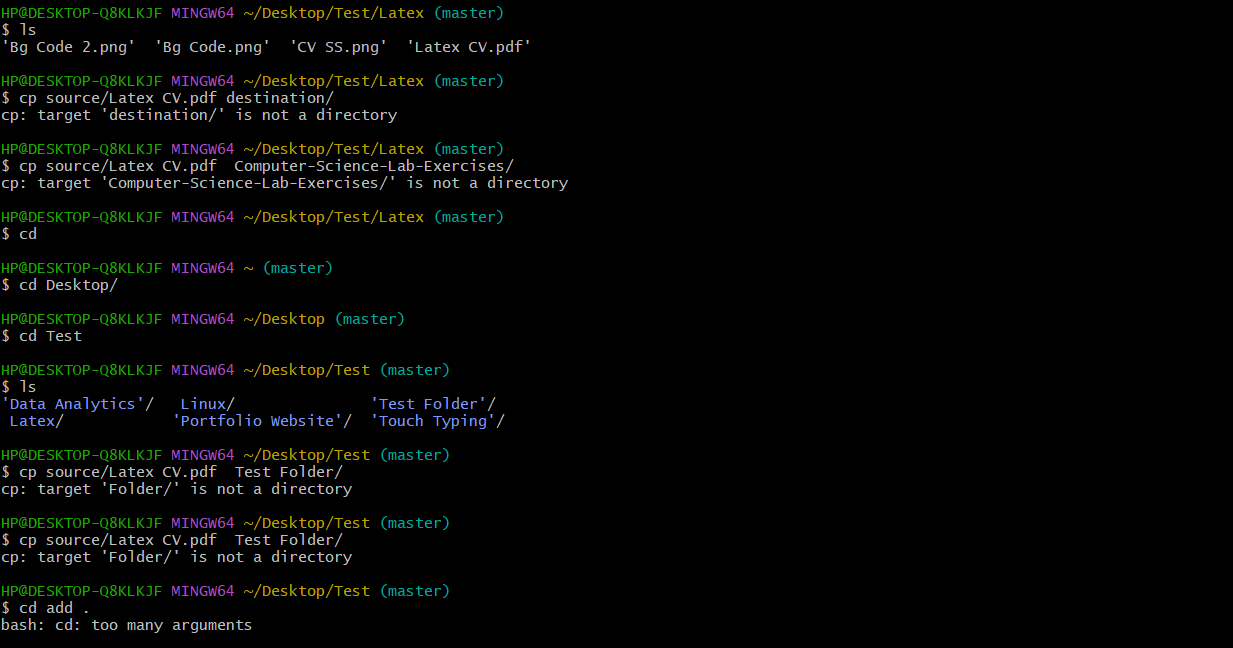
\includegraphics[width=225,height=0.35\textheight]{Git 2.png}
 
 \end{tabular}

\subsection{Git Hub}
\rule{\textwidth}{0.1pt}
\subsubsection{Introduction}
GitHub is a for-profit company that offers a cloud-based Git repository hosting service. Essentially, it makes it a lot easier for individuals and teams to use Git for version control and collaboration.

GitHub’s interface is user-friendly enough so even novice coders can take advantage of Git. Without GitHub, using Git generally requires a bit more technical savvy and use of the command line.

GitHub is so user-friendly, though, that some people even use GitHub to manage other types of projects – like writing books.

Additionally, anyone can sign up and host a public code repository for free, which makes GitHub especially popular with open-source projects.
\subsubsection{Explanation}
In this exercise the reporter has successfully create his Github profile. The reporter has reposit all the exercise done in the module of Computer Science Lab trough the repository here is the user Github Link under.
\subsubsection{GitHub:}
Here is the Reporter GitHub Link: \fontfamily{\sfdefault}\selectfont \color{black}
   \href{https://github.com/Hassan-Muhammad-Yousuf}{\raisebox{-0.1\height}\faGithub\ {Hassan-Muhammad-Yousuf}} \\



\section{Conclusion}

\rule{\textwidth}{0.1pt}
    \noindent 
    \justifying A comprehensive study summarizes the findings of a comprehensive study concentrating on the significance of understanding how to manage complex problems in the field of computer science by utilizing a variety of technical resources when working on various software development projects. It is necessary to be familiar with a variety of techniques using different tools, such as Linux, Touch Typing, HTML, CSS, LaTeX, GitHub etc., to guarantee the efficient operation of software development initiatives. By analyzing the results of several exercises, the efficacy, performance, and practical applications of computer software are evaluated. As an illustration, the software development process may involve designing, developing, testing, and deploying software. Complex problems that can be better analyzed and comprehended through solution-based exercises. Additionally, developers can use other techniques to identify and correct code errors. This ensures that the software conforms to the specified requirements and performs as expected.\\
    
    The majority of this report is devoted to application software that is in high demand across numerous industries. This study continues to concentrate on GitHub's open network of open-source projects and the collaborative and computational benefits that result. Other problem identifies potential software errors or flaws, allowing developers to repair them before releasing the software. This ensures that the software functions correctly and meets the user's requirements. In addition, the use of diagnostic tools can help identify potential software issues in advance, thereby reducing the likelihood that errors will occur once the software is deployed.

\end{document}
